\documentclass[xcolor=dvipsnames]{beamer} 
\usepackage{ulem}
\usepackage{tabularx}
\usepackage{xcolor,colortbl}

\newcommand{\mc}[2]{\multicolumn{#1}{c}{#2}}
\definecolor{Gray}{gray}{0.85}
\definecolor{LightGreen}{rgb}{1,0.88,1}

\newcolumntype{a}{>{\columncolor{Gray}} X }
\newcolumntype{b}{>{\columncolor{white}} X }


% This file is a solution template for:

% - Talk at a conference/colloquium.
% - Talk length is about 20min.
% - Style is ornate.

% Copyright 2004 by Till Tantau <tantau@users.sourceforge.net>.
%
% In principle, this file can be redistributed and/or modified under
% the terms of the GNU Public License, version 2.
%
% However, this file is supposed to be a template to be modified
% for your own needs. For this reason, if you use this file as a
% template and not specifically distribute it as part of a another
% package/program, I grant the extra permission to freely copy and
% modify this file as you see fit and even to delete this copyright
% notice. 


\mode<presentation>
{
  %\usetheme{boxes}
  %\usecolortheme{seagull}
  % or ...

  \setbeamercovered{transparent}
  % or whatever (possibly just delete it)

    \usecolortheme[named=OliveGreen]{structure} 
    \usetheme[height=7mm]{Rochester} 
    \setbeamertemplate{items}[ball] 
    \setbeamertemplate{blocks}[rounded][shadow=true]
}


\usepackage[czech]{babel}
% or whatever

\usepackage[utf8]{inputenc}
% or whatever

\usepackage{hyperref}
%\definecolor{links}{HTML}{2A1B81}
\hypersetup{colorlinks,linkcolor=OliveGreen,urlcolor=OliveGreen}

\usepackage{times}
% \usepackage[T1]{fontenc}
% Or whatever. Note that the encoding and the font should match. If T1
% does not look nice, try deleting the line with the fontenc.



% If you have a file called "university-logo-filename.xxx", where xxx
% is a graphic format that can be processed by latex or pdflatex,
% resp., then you can add a logo as follows:

\pgfdeclareimage[height=1.cm]{conference-logo}{images/logo_cost.png}
\pgfdeclareimage[height=1.cm]{pywps}{images/pywps.png}
\logo{\pgfuseimage{conference-logo}}



% Delete this, if you do not want the table of contents to pop up at
% the beginning of each subsection:
\mode<presentation>
\AtBeginSection[]
{
%\logo{\pgfuseimage{conference-logo}}
  \begin{frame}<beamer>{TOC}
    \tableofcontents[currentsection,currentsubsection]
  \end{frame}
}


% If you wish to uncover everything in a step-wise fashion, uncomment
% the following command: 

%\beamerdefaultoverlayspecification{<+->}


\title{PyWPS -- Project status and demo}

\subtitle {}

\author[J. Čepický] % (optional, use only with lots of authors)
{Jáchym~Čepický\inst{1}}
% - Give the names in the same order as the appear in the paper.
% - Use the \inst{?} command only if the authors have different
%   affiliation.

\institute % (optional, but mostly needed)
{
  \inst{1}%
  Geosense s.r.o.
  \url{http://geosense.cz}\\
}
  
% - Use the \inst command only if there are several affiliations.
% - Keep it simple, no one is interested in your street address.

\date[] % (optional, should be abbreviation of conference name)
{WPS Workshop}
% - Either use conference name or its abbreviation.
% - Not really informative to the audience, more for people (including
%   yourself) who are reading the slides online



\begin{document}

%\begin{abstract}
%\end{abstract}

\begin{frame}
  \titlepage
  \begin{center}
    
\includegraphics[width=2cm]{images/pywps.png}
  \end{center}
\end{frame}

%\begin{frame}{TOC}
%  \tableofcontents
%  % You might wish to add the option [pausesections]
%\end{frame}

\begin{frame}{Jachym Cepicky}
  \begin{columns}
  \column{0.7\textwidth}
    \begin{itemize} 
        \item Forester
        \item OpenSource GIS developer (former user) - GRASS, OpenLayers, PyWPS, \dots
        \item Member of Board of directors of Open Source Geospatial Foundation (\href{http://osgeo.org}{OSGeo.org})
        \item \href{http://twitter.com/jachymc}{@jachymc}
            \href{http://les-ejk.cz}{http://les-ejk.cz}
            \href{http://www.openstreetmap.org/user/jachymc}{http://www.openstreetmap.org/user/jachymc}
    \end{itemize}
    \column{0.3\textwidth}
    
\includegraphics[width=0.75\textwidth]{images/profil2.jpg}
\end{columns}
\end{frame}

\section{About PyWPS}
%%%%%%%%%%%%%%%%%

\begin{frame}{What is PyWPS}
\begin{itemize} 
    \item OGC WPS on the Server
    \item Since 2006
    \item Python
    \item \url{http://pywps.wald.intevation.org}
    \item \url{http://github.org/geopython/pywps}
\end{itemize} 
\end{frame}

\begin{frame}{PyWPS - what it is NOT}
    \alert{
        \begin{itemize}
            \item PyWPS is no analytical tool or engine. It does not perform any type of geospatial calculation.
                \pause
            \item PyWPS is not special XML parser or generator. It does not validate your GMLs against given schemas (yet), it does not build GML from Python objects.
                \pause
            \item It is not complicated
        \end{itemize}
    }
\end{frame}

\begin{frame}{Keywords}
    \begin{center}
        \only<2>{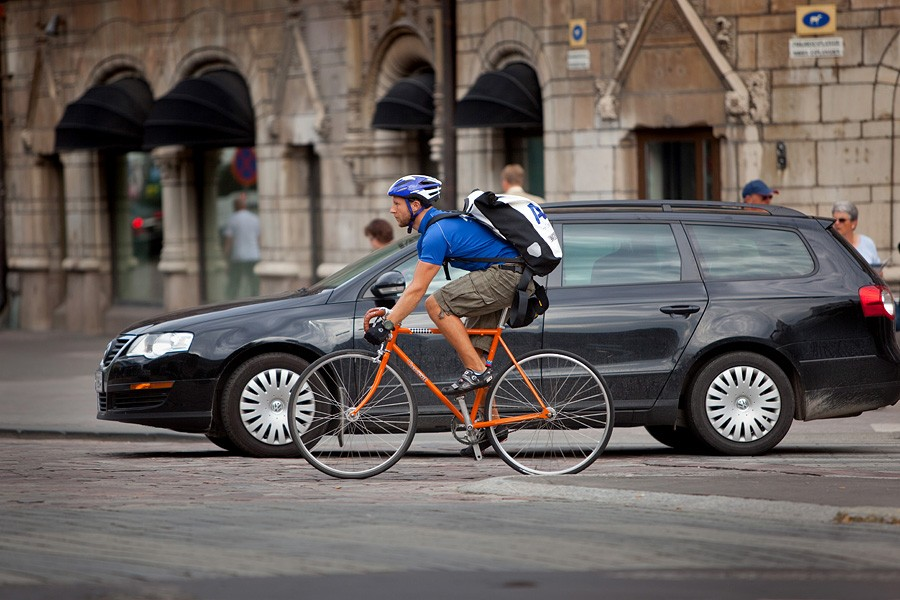
\includegraphics[width=\textwidth]{images/bike-car.jpg}\\
            rather bike, then a car}
        \only<3>{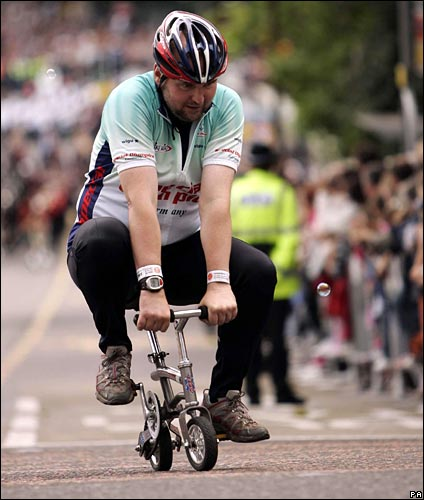
\includegraphics[height=7cm]{images/small-bike.jpg}\\
            \#small}
        \only<4>{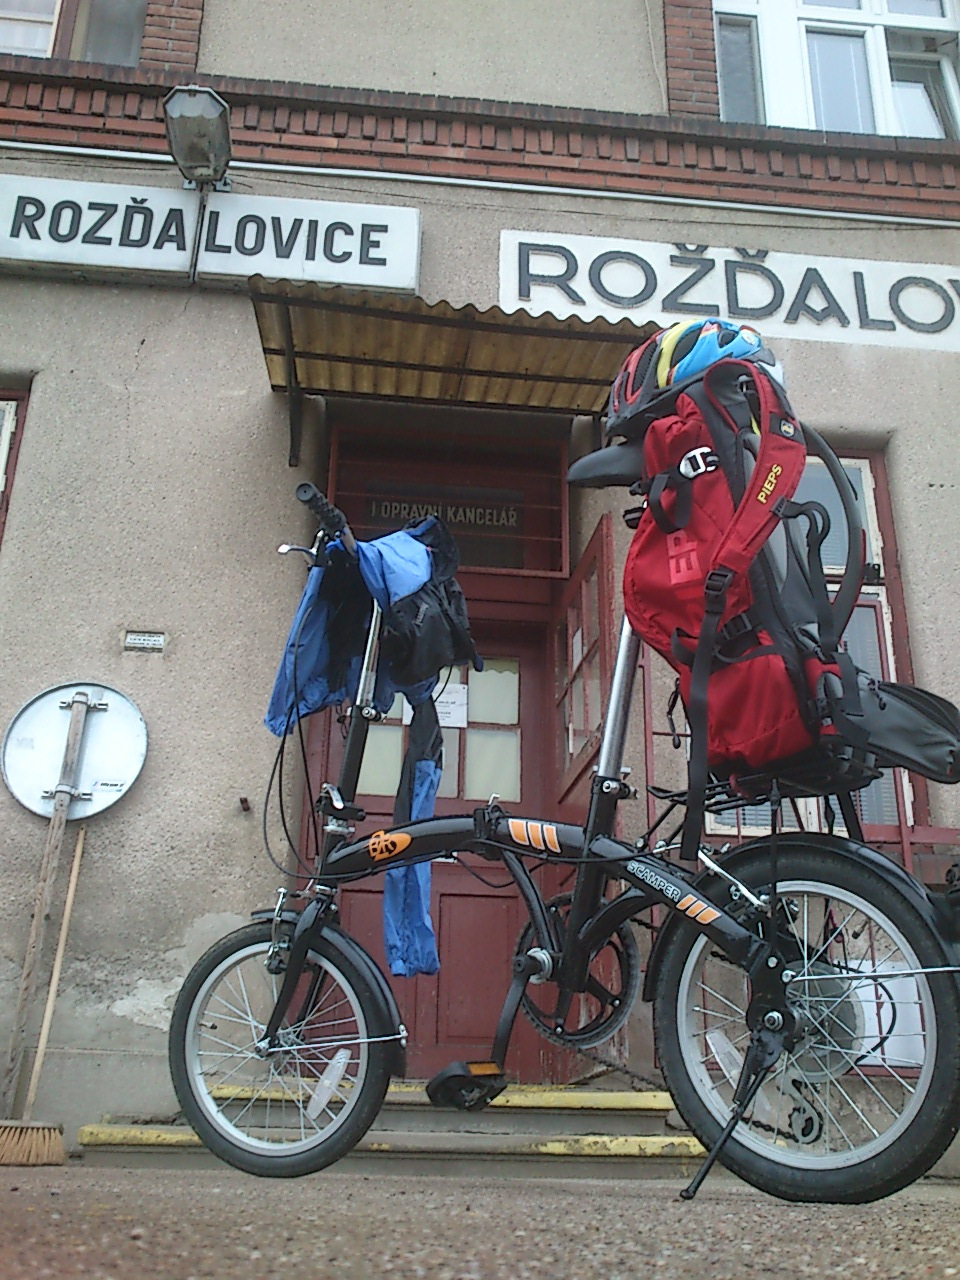
\includegraphics[height=7cm]{images/modular-bike.jpg}\\
            \#modular}
        \only<5>{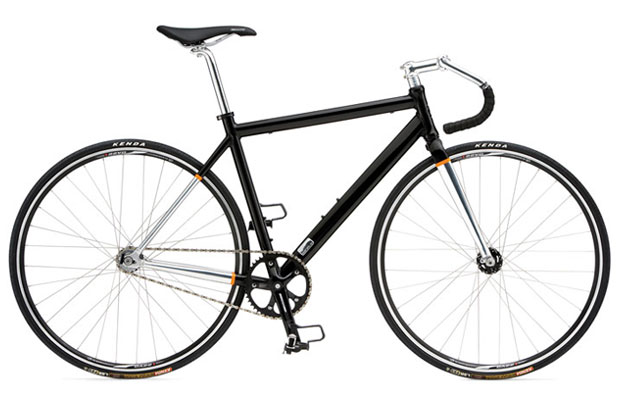
\includegraphics[width=\textwidth]{images/fast-bike.jpg}\\
            \#fast
        }
        \only<6>{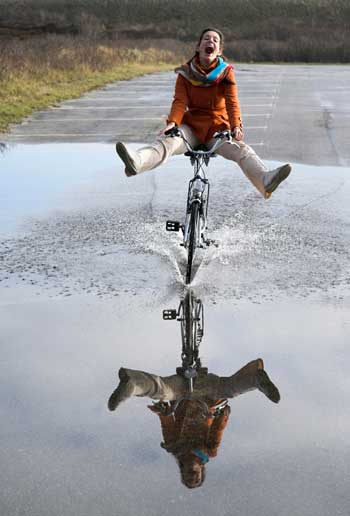
\includegraphics[height=7cm]{images/easy-bike.jpg}\\
            \#easy
        }
        \only<7>{
\includegraphics[height=7cm]{images/slick-bike.jpg}\\
            \#slick}
        \only<8>{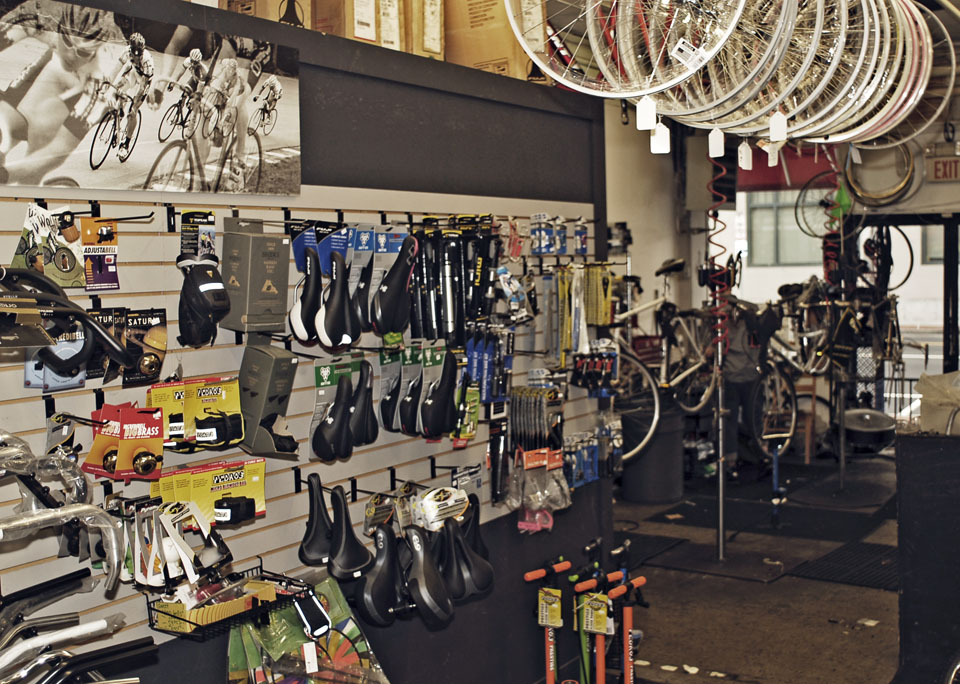
\includegraphics[height=7cm]{images/bike-accessories.jpg}\\
        \#accessories (GRASS, GDAL, Shapely, \#python)}
    \end{center}
\end{frame}

\begin{frame}{History of PyWPS}
\begin{description}
    \item[2006-11-10 version 1.0.0] Web User Interface for WPS (Embrio).
    \item[2007-10-08 version 2.0.0] New version improved stability, {\em Process} class, OpenLayers 2.x.
    \item[2008-11-06 version 3.0.0] New code structure, implementation of WPS 1.0.0
    \item[2009-06-01 version 3.1.0] New generic JavaScript WPS Client library and more.
    \item[2011-09-06 version 3.2.0] MapServer
    \item[2013] Moved to GitHub \url{http://github.com/geopython/pywps}
    \item[2013-5] FOSS4G-CEE 2013, Bucharest, Started to work on PyWPS-4
\end{description}
\end{frame}

\begin{frame}{How does it work}
\begin{center}
    \only<1>{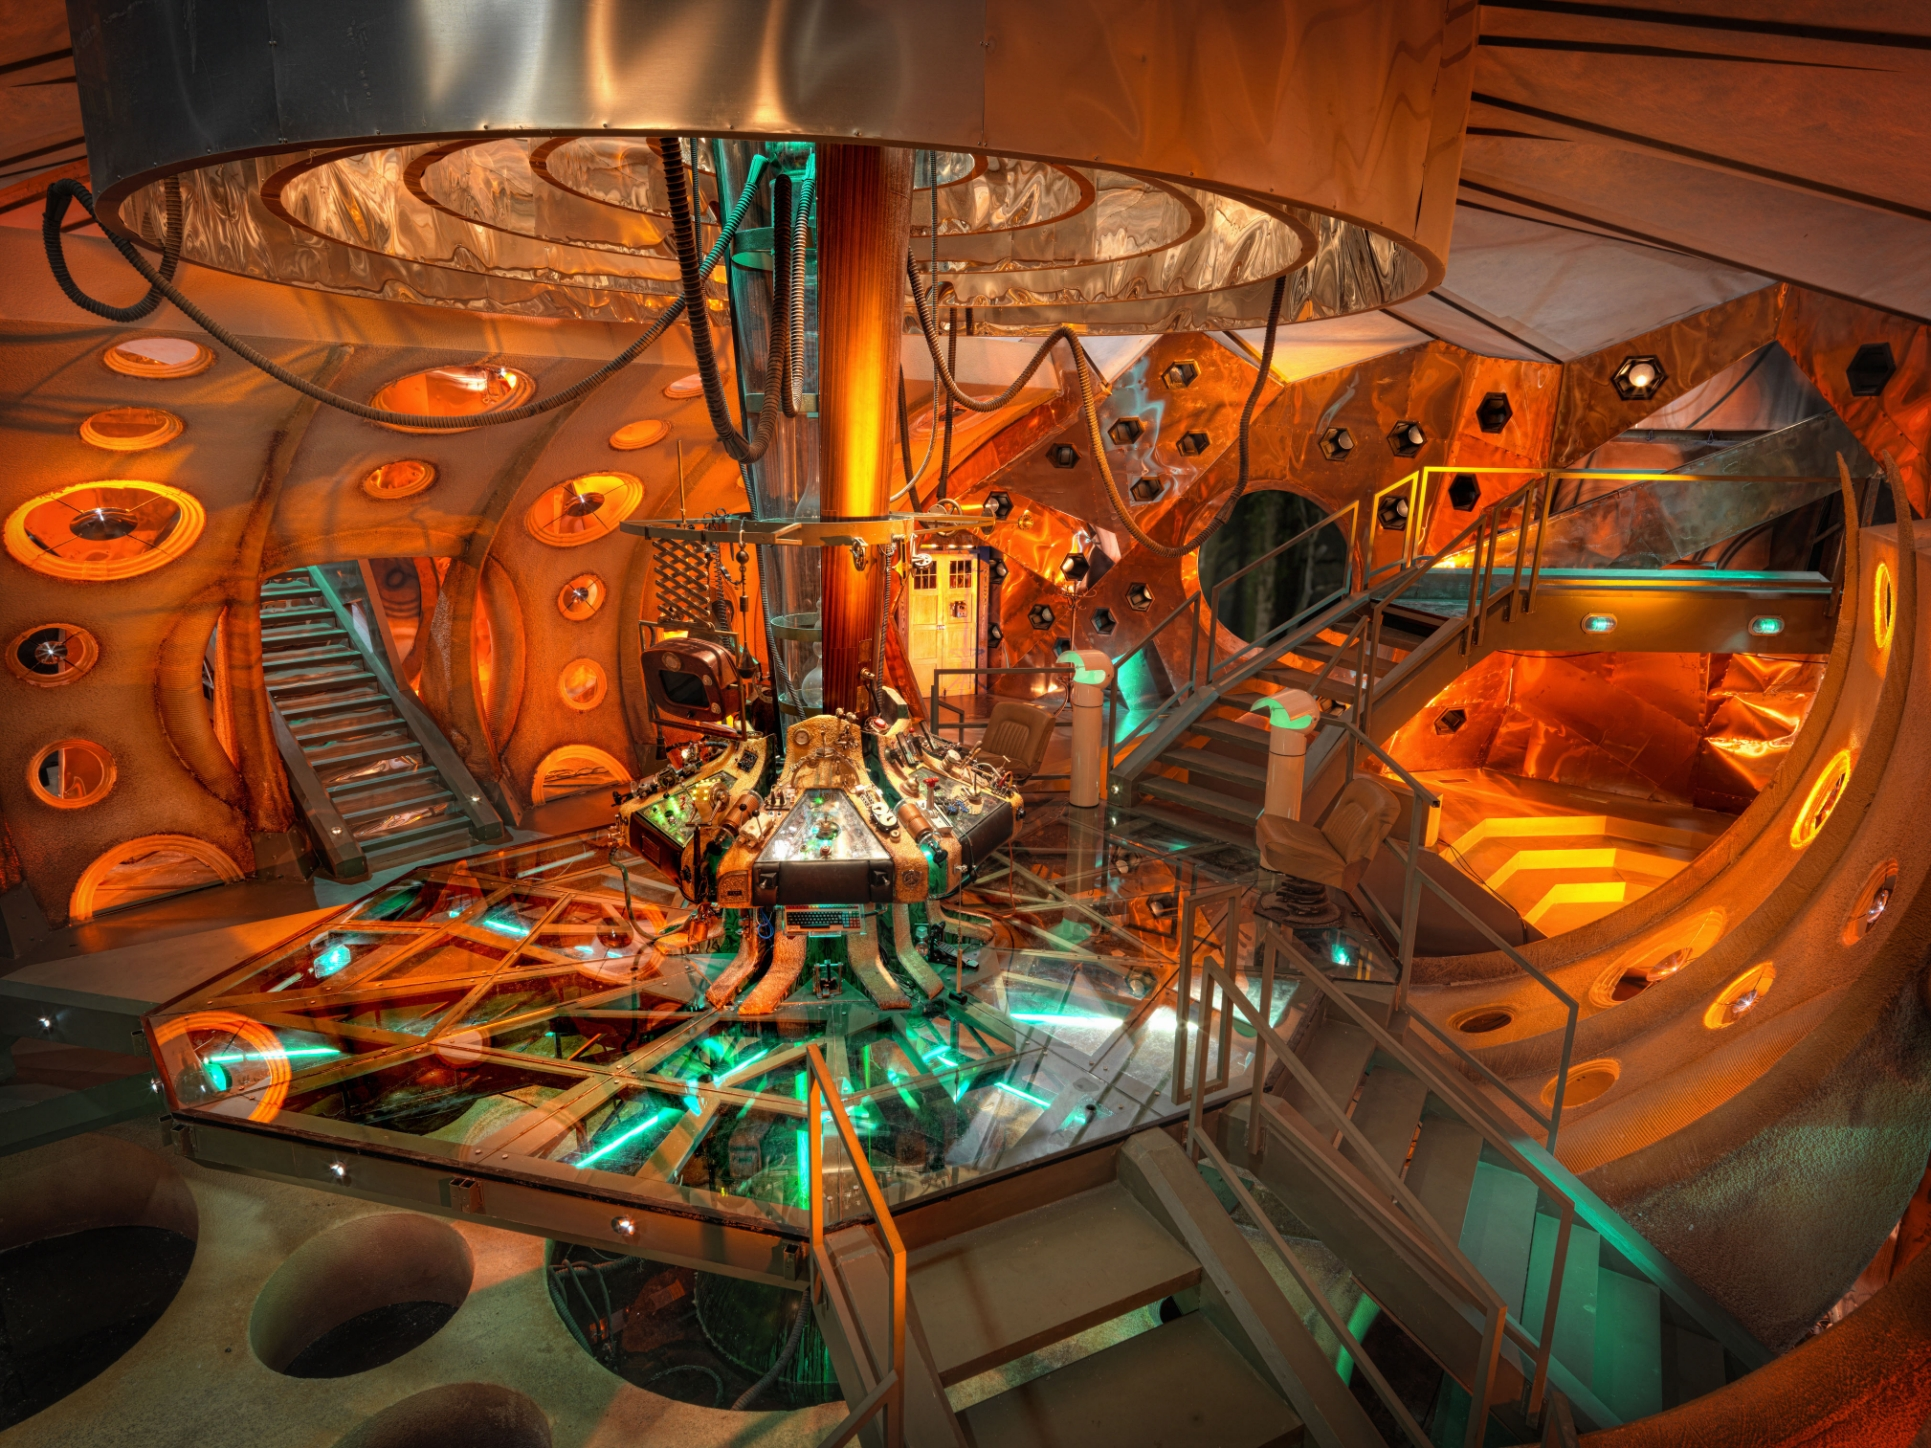
\includegraphics[width=\textwidth]{images/tardis_interior.jpg}\\
    Time machine / climate change model}
    \only<2>{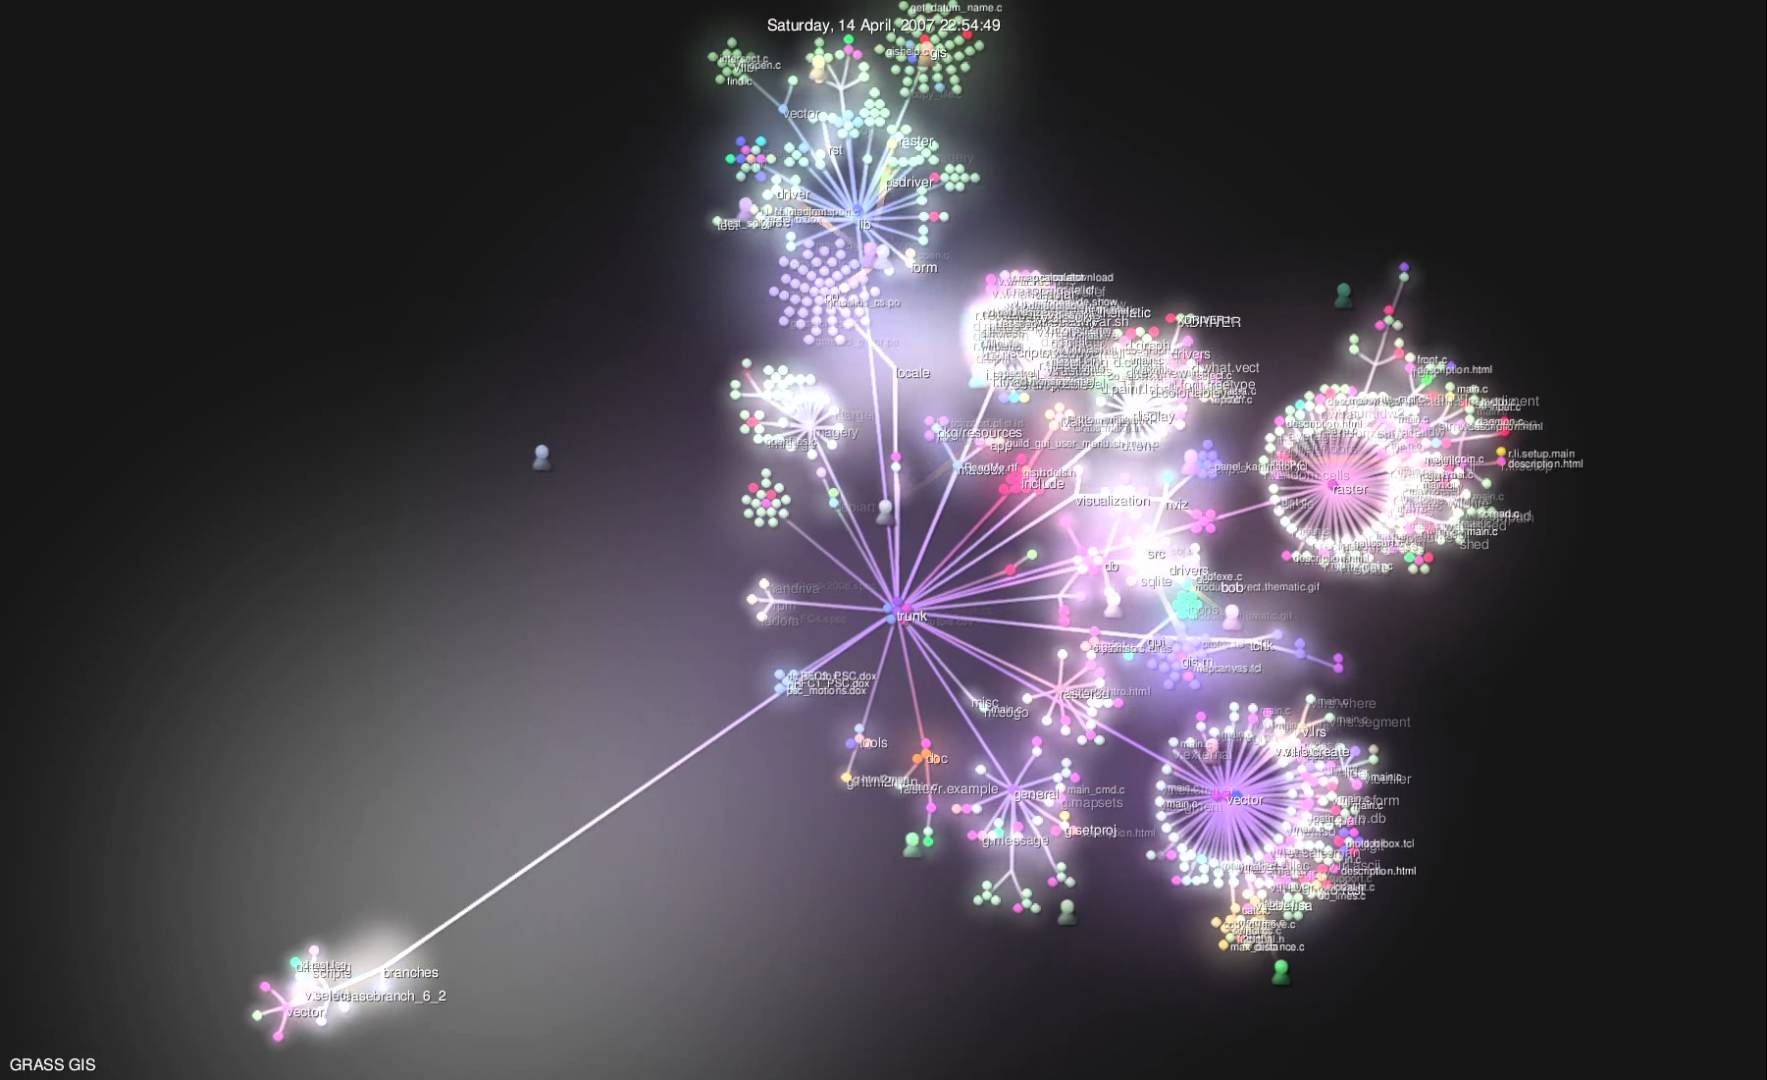
\includegraphics[width=\textwidth]{images/maxresdefault.jpg}\\
    Internet, sharing}
    \only<3>{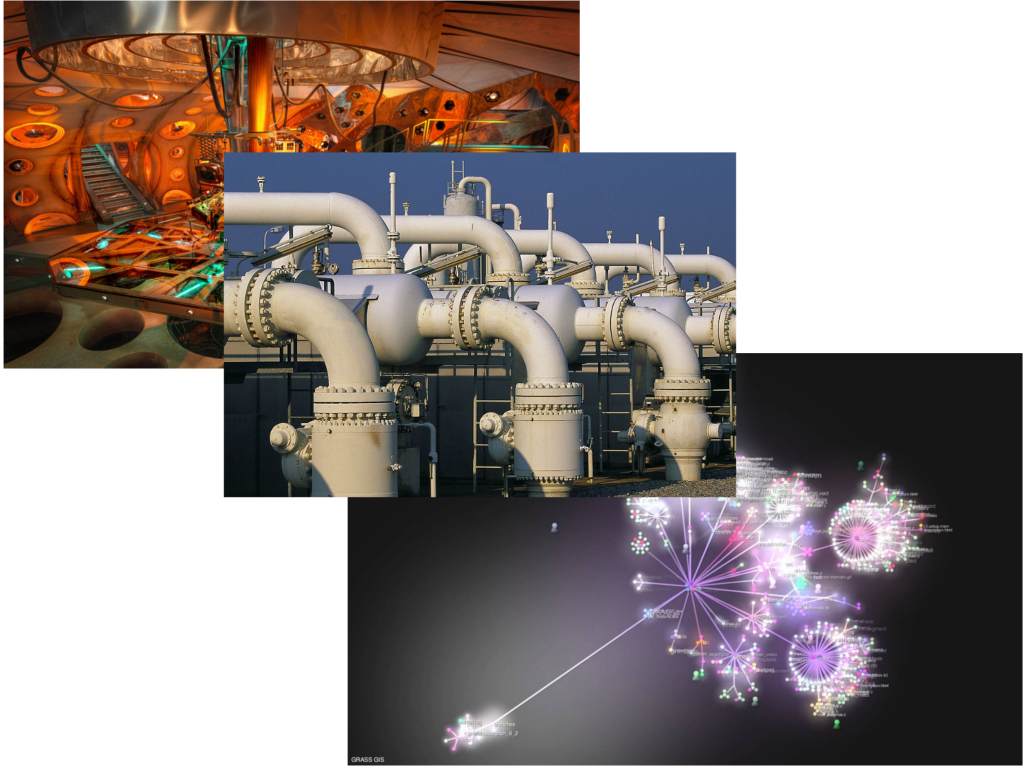
\includegraphics[width=\textwidth]{images/pywps-pipes.png}}
    \only<4>{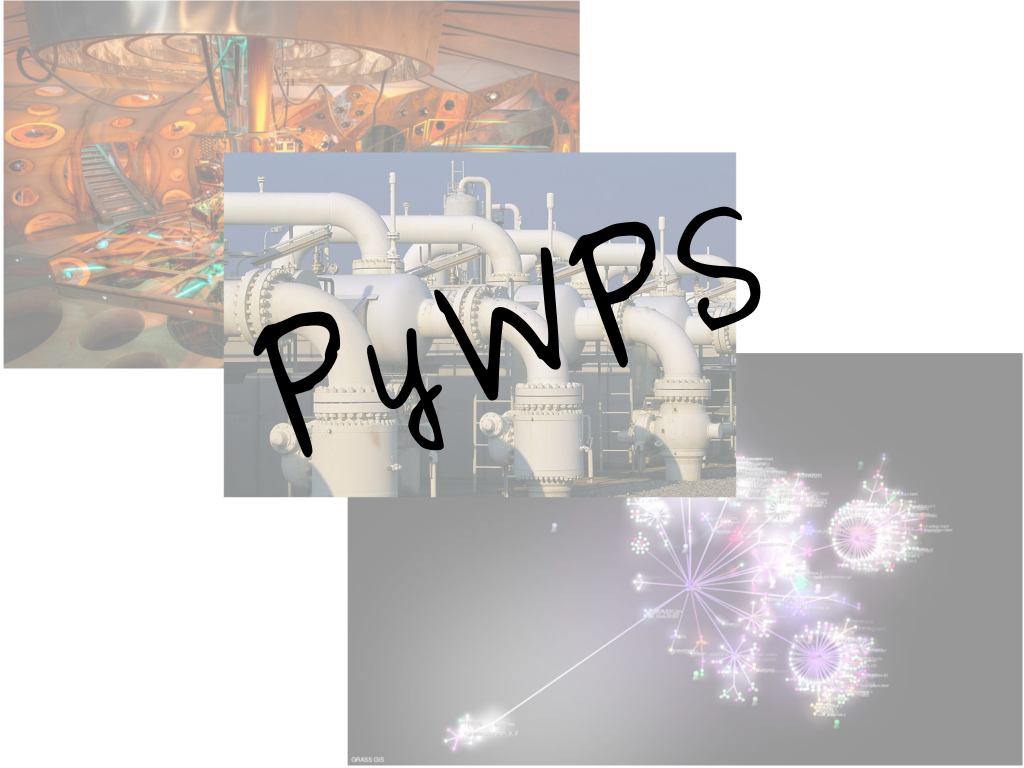
\includegraphics[width=\textwidth]{images/pywps-pipes-pywps.png}}
    \only<5>{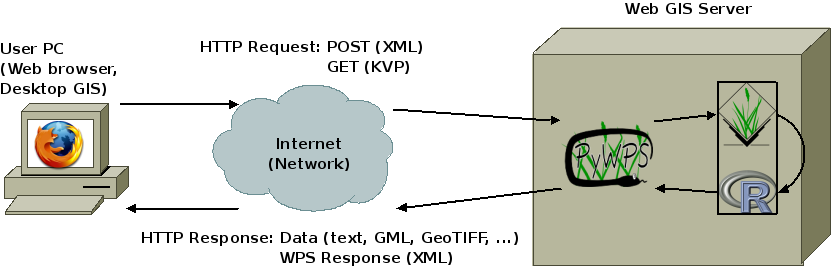
\includegraphics[width=\textwidth]{images/pywps-schema.png}}
    \only<6>{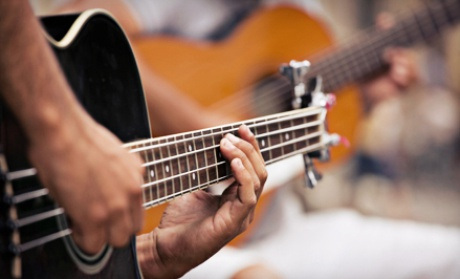
\includegraphics[width=\textwidth]{images/c460x279.jpg}\\
    One process}
    \only<7>{
\includegraphics[width=\textwidth]{images/four-handed-guitar.jpg}\\
    Two processes}
    \only<8>{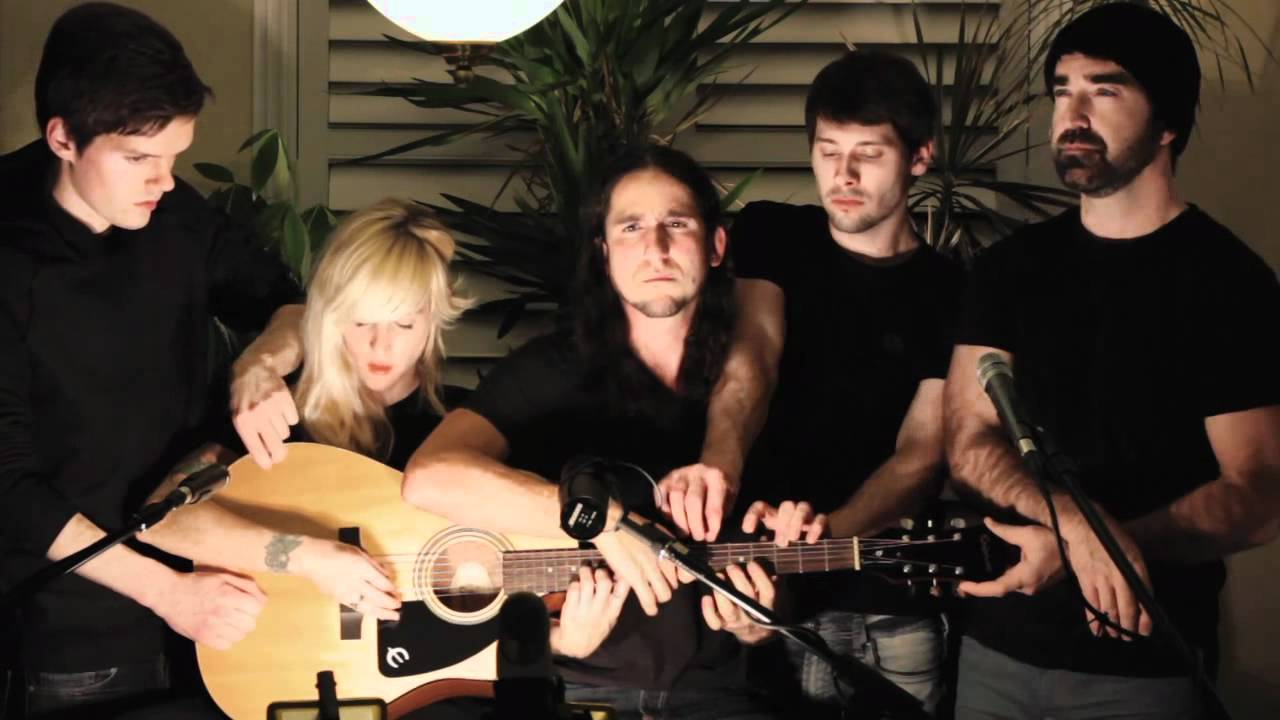
\includegraphics[width=\textwidth]{images/5-guitar.jpg}\\
    Process chain}
\end{center}
\end{frame}

\section{Code}
%%%%%%%%%%%%%%%%%

\scriptsize{
\begin{frame}[fragile]
\frametitle{Talk is cheap. Show me the code}
%\thispagestyle{empty}
\begin{semiverbatim}
\uncover<1->{
1 from pywps.Process import WPSProcess                                
2 from osgeo import ogr
3 import types
4 [...]}
\uncover<2->{5         WPSProcess.__init__(self,
6             identifier = "ogrbuffer", # must be same, as filename
7              title="Buffer process using OGR")
8 [...]}
\uncover<3->{9       self.data = self.addComplexInput(identifier = "data")
10      self.size = self.addLiteralInput(identifier="size") 
11      self.output =self.addComplexOutput(identifier="buffer") 
}
\end{semiverbatim}
\end{frame}

\begin{frame}[fragile]
\frametitle{Talk is cheap. Show me the code}
\begin{semiverbatim}
\uncover<1->{
10    def execute(self):
11
12       inSource = ogr.Open(self.data.getValue())
13       inLayer = inSource.GetLayer()
14
15       [...]
16       outLayer = outSource.CreateLayer(
17           out,None,ogr.wkbUnknown)
18
19       [...]}
\uncover<2->{
20      while index < featureCount:
21          self.status.set("Calculating buffer for feature %d from %d" % (index+1,featureCount),
22                  (100*(index+1)/featureCount*1.0))
23          [...]
24          inGeometry = inFeature.GetGeometryRef()
25
26          # make the buffer
27          buff = inGeometry.Buffer(float(self.size.getValue()))
28
29          [...]
30      self.output.setValue(out)
31      return}
\end{semiverbatim}
\end{frame}
} % /scriptsize

\begin{frame}{What can be connected}
\begin{itemize}
    \item Python* (GDAL/OGR, GRASS, MapServer, Shapely, Fiona, R, PostGIS, \dots)
    \item Jython - Java* (GeoTools, JTS, GeoServer, \dots)
    \item Any batch file
\end{itemize}
\end{frame}

\begin{frame}{Tools, which are tested with PyWPS}
\begin{itemize}
    \item GRASS (GRASS-WPS interface, Sören Gebert)
    \item R
    \item Taverna (WPS-WSDL orchestration, Jorge de Jesus)
    \item MapServer (output generation using OGC OWS, still concept)
\end{itemize}
\end{frame}

\section{PyWPS 4}
%%%%%%%%%%%%%%%%%

\begin{frame}{Bright future}
\begin{itemize}
    \item Started from scratch
    \item Use Python 2.7 (for future 3.0 migration)
    \item Try different interpreters of Python (pypy)
    \item Easy parsing with lxml
    \item Prepare for next WPS version
    \item Change of the whole process concept
\end{itemize}
\end{frame}

\begin{frame}{PyWPS 4}
    \begin{center}
        \only<1>{
        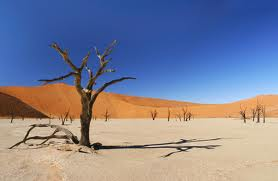
\includegraphics[height=7cm]{images/desert.jpg}\\
            \#geopython 2006
        }
        \only<2>{
        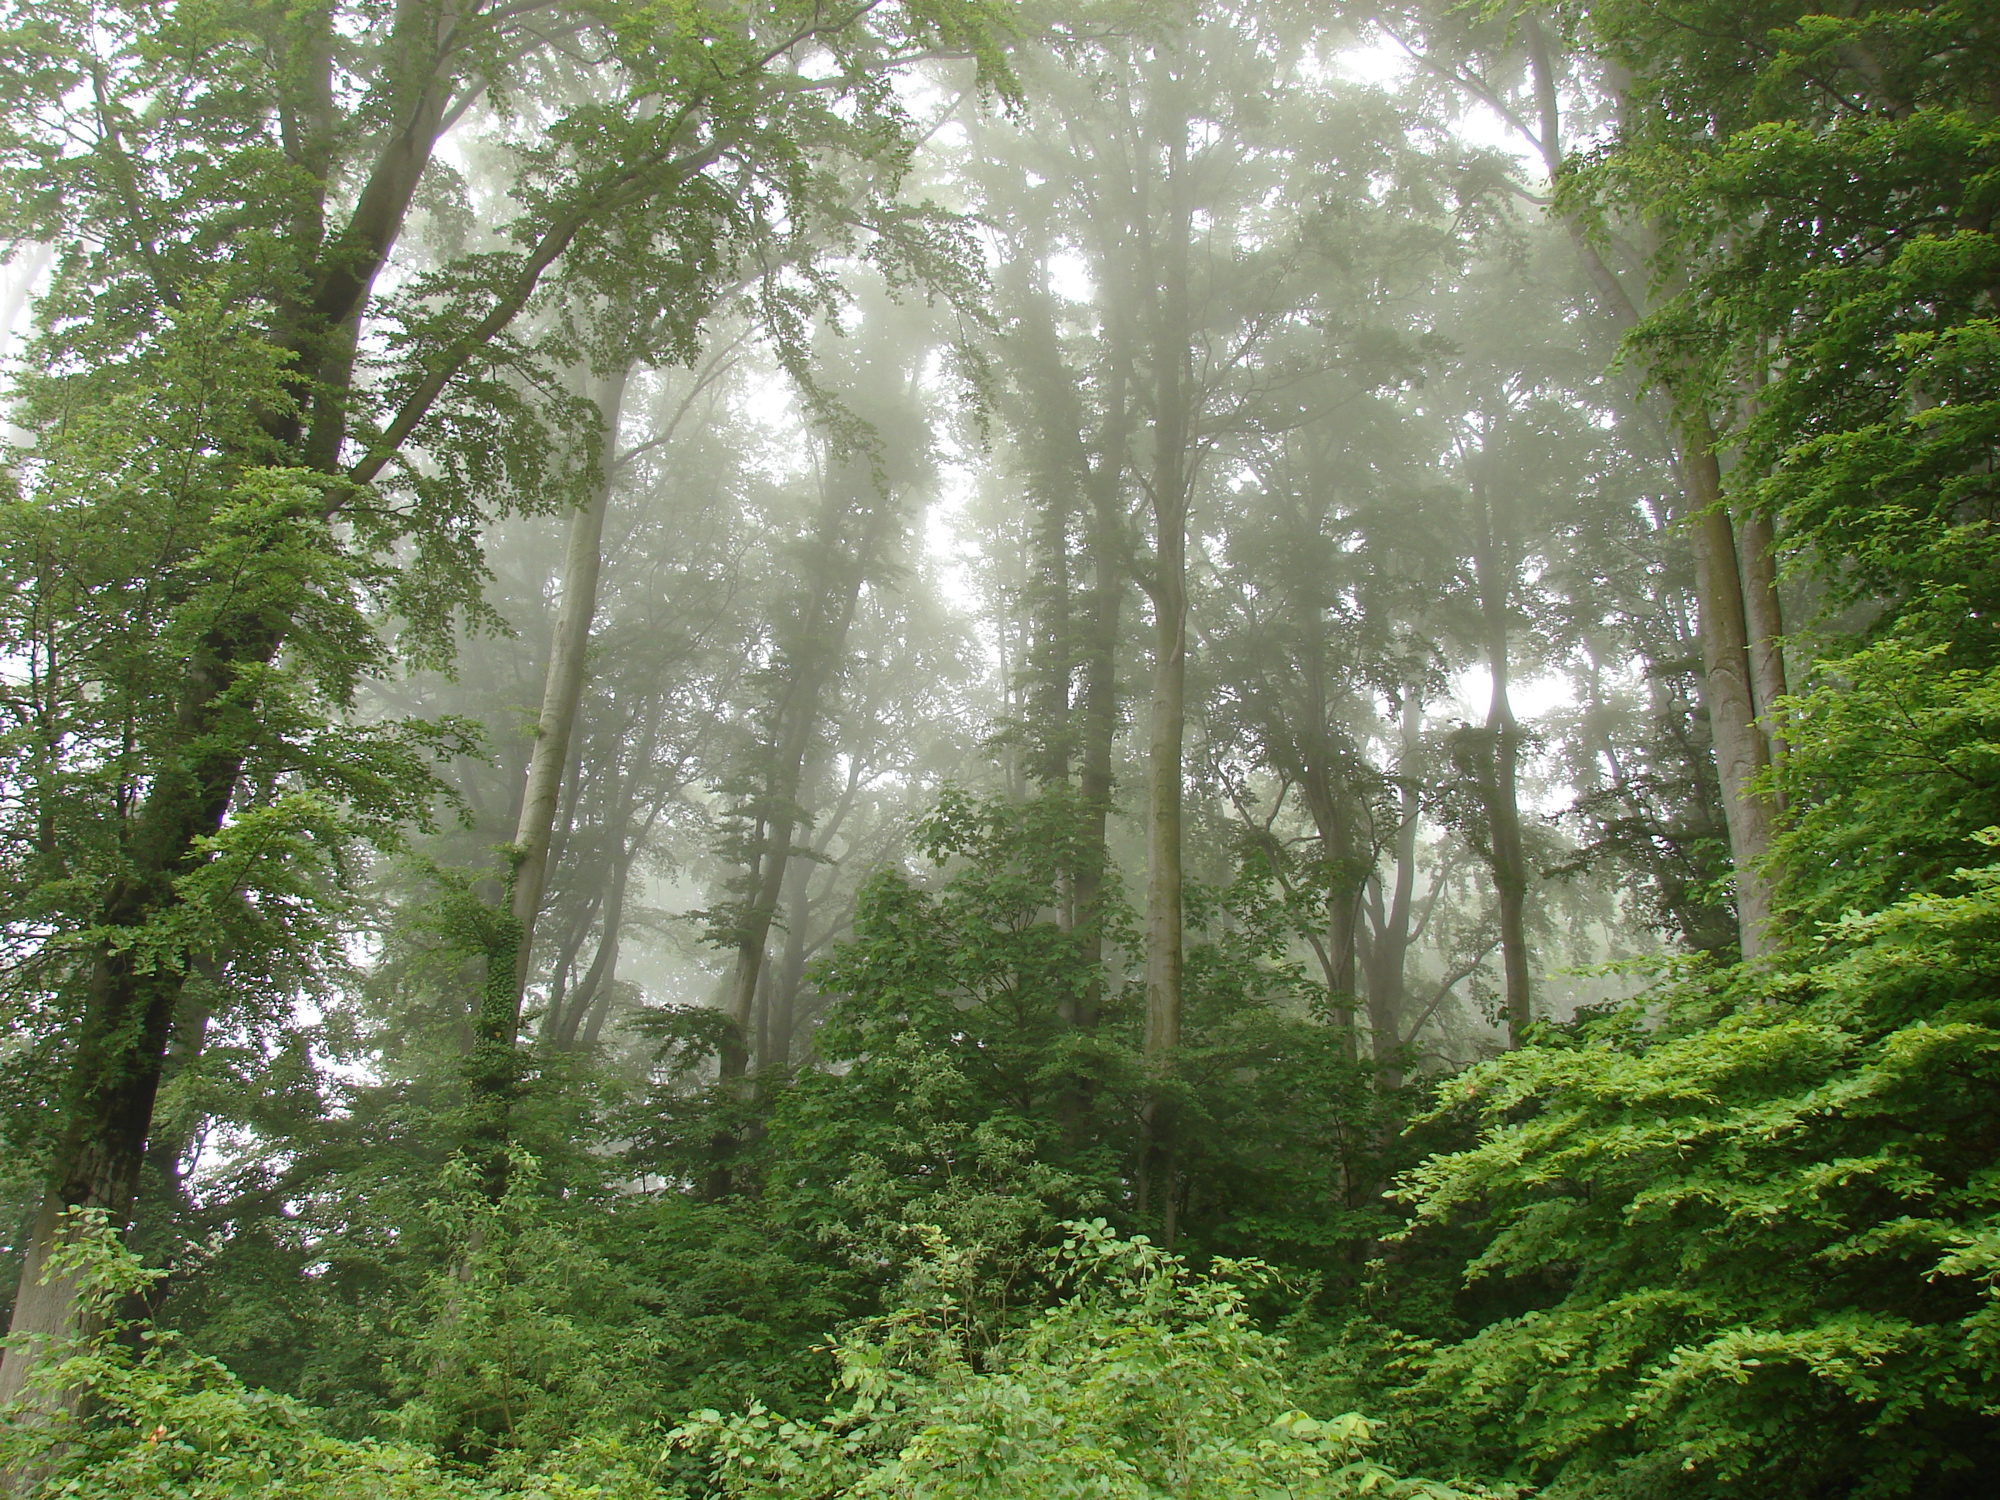
\includegraphics[height=7cm]{images/prales.jpg}\\
            \#geopython 2013
        }
    \end{center}
\end{frame}

\begin{frame}
    \begin{itemize}
        \item lxml \url{http://lxml.org}
        \item GRASS-WPS, GRASS-Python
        \item Werkzeug \url{http://werkzeug.pocoo.org/}
        \item Python 3
        \item Django
        \item MapServer for output generation
        \item Respect to new OGC WPS 2.0.0 features
        \item \dots
    \end{itemize}
\end{frame}

\section*{Conclusion}
\begin{frame}
    Happy processing!\\
    ~
    \\
    jachym.cepicky@gmail.com \\
    http://les-ejk.cz \\
    @jachymc\\
    ~
    \\
    \url{http://github.org/jachym/pywps-4}\\
    \url{http://pywps.wald.intevation.org}
\end{frame}

\end{document}
